\documentclass[a4paper, 12pt, titlepage]{article}

% Including needed packages
\usepackage[margin=2cm]{geometry}
\usepackage{amsmath}
\usepackage{amssymb}
\usepackage{amsthm}
\usepackage{graphicx}
\usepackage{subfig}
\usepackage{float}
\usepackage{makecell}

\newcommand{\norm}[1]{\lVert#1\rVert}

\title
{{\em Machine learning 2}\\
Exercise sheet 8}
\author{FLEISCHMANN Kay, Matrnr: 352247\\
	ROHRMANN Till, Matrnr: 343756}
\date{\today}

\begin{document}

\maketitle

\section{Weighted Degree Kernels}

The weighted degree kernel is defined as:
\begin{eqnarray}
	k(x_i,x_j) &=& \sum_{m=1}^M \beta_m \sum_{n=1}^{N-m+1} \boldsymbol{I}\left(u_{m,n}(x_i)=u_{m,n}(x_j)\right)
\end{eqnarray}

where $u_m,n(x)$ is a string of length $m$ which starts at position $n$ in sequence $x$. 
$\boldsymbol{I}(\cdot)$ is the indicator function.
$\beta_m=2\frac{M-m+1}{M(M+1)}$ is used for weighting.

\begin{proof}[Show that $k(\cdot,\cdot)$ is a positive semi-definite symmetric kernel]
First we show that $k(\cdot,\cdot)$ is symmetric:
Given two strings $x$ and $y$ of length $N$.
\begin{eqnarray*}
	k(x,y) &=& \sum_{m=1}^M\beta_m\sum_{n=1}^{N-m+1}\boldsymbol{I}\left(u_{m,n}(x)=u_{m,n}(y)\right)\\
	&=& \sum_{m=1}^M\beta_m\sum_{n=1}^{N-m+1}\boldsymbol{I}\left(u_{m,n}(y)=u_{m,n}(x)\right)\\
	&=& k(y,x)
\end{eqnarray*}

Now we only have to show that $k(\cdot,\cdot)$ is positive semi-definite, that is to say $\forall v\in \mathbb{R}^L: v^TKv\ge0$ where $(K)_{i,j}=k(x_i,x_j)$ for some arbitrary $x_i$ with $1\le i\le L$.

\begin{eqnarray}
	v^TKv &=& \sum_{i,j=1}^L v_i k(x_i,x_j) v_j \nonumber \\
	&=&  \sum_{i,j=1}^L v_i \left(\sum_{m=1}^M\beta_m\sum_{n=1}^{N-m+1}\boldsymbol{I}\left(u_{m,n}(x_i)=u_{m,n}(x_j)\right)\right)  v_j \label{eq:psd}
\end{eqnarray}
Since our alphabet $\mathcal{A}$ of the strings is finite, we can reformulate $\boldsymbol{I}\left(u_{m,n}(x_i)=u_{m,n}(x_j)\right)$:
\begin{eqnarray}
	\boldsymbol{I}\left(u_{m,n}(x_i)=u_{m,n}(x_j)\right) &=& \sum_{w\in\mathcal{A}^m} \boldsymbol{I}\left(u_{m,n}(x_i)=w\right)\cdot \boldsymbol{I}\left(u_{m,n}(x_j)=w\right) \label{eq:indicator}
\end{eqnarray}

Inserting equation \eqref{eq:indicator} into equation \eqref{eq:psd} we obtain:
\begin{eqnarray*}
	\eqref{eq:psd} &=& \sum_{i,j=1}^L v_i \left(\sum_{m=1}^M\beta_m\sum_{n=1}^{N-m+1}\left(\sum_{w\in\mathcal{A}^m} \boldsymbol{I}\left(u_{m,n}(x_i)=w\right)\cdot \boldsymbol{I}\left(u_{m,n}(x_j)=w\right)\right)\right)  v_j\\
	&=& \sum_{m=1}^{M}\beta_m\sum_{n=1}^{N-m+1}\sum_{w\in\mathcal{A}^m}\sum_{i,j=1}^L v_i \boldsymbol{I}(u_{m,n}(x_i)=w)\cdot \boldsymbol{I}(u_{m,n}(x_j)=w) v_j\\
	&=& \sum_{m=1}^{M}\beta_m\sum_{n=1}^{N-m+1}\sum_{w\in\mathcal{A}^m}\left(\sum_{i=1}^L v_i \boldsymbol{I}(u_{m,n}(x_i)=w)\right) \left(\sum_{j=1}^L v_j\boldsymbol{I}(u_{m,n}(x_j)=w)\right) \label{eq:psd2}
\end{eqnarray*}

In equation \eqref{eq:psd2} we used the fact that the double sum can be expressed by the product of two sums (by simply factoring out).

\begin{eqnarray*}
	\eqref{eq:psd2} &=& \sum_{m=1}^{M}\underbrace{\beta_m}_{\ge 0}\sum_{n=1}^{N-m+1}\sum_{w\in\mathcal{A}^m}\underbrace{\left(\sum_{i=1}^L v_i \boldsymbol{I}(u_{m,n}(x_i)=w)\right)^2}_{\ge 0} \\
	&\ge& 0
\end{eqnarray*}

Thus we have just proved that $k(\cdot,\cdot)$ is positive semi-definite and together with the fact that it's symmetric the proposition is proven.
Due to the Mercer's theorem it further holds that the kernel function $k(\cdot,\cdot)$ is the inner product of two vectors transformed into an inner product space.
\end{proof}

\section{SVM light}

In this sub task we were supposed to apply SVMlight onto weighted degree kernels and evaluate the performance.
We executed SVMlight for the parameters $M=1,2,3$ and the regularization constant $C=0.001,0.01,0.1,1,10$.

Figure \ref{fig:ptacc} contains the plots of the prediction accuracy on the testing and training data set depending on the regularization parameter $C$ for the different $M$ values.
For all values of $M$ we can observe that the prediction accuracy on the training data set converges to $1$ with an increasing $C$.
This is due to the fact that the use of slack variables is more highly penalized and thus forcing the optimization procedure to minimize the classification error at the cost of a smaller margin.
However, we can also see by observing the prediction accuracy on the testing data set that the accuracy degrades with high $C$ values after reaching a maximum.
This indicates that the SVM overfits to the training data set and thus high accuracies on the training data set do not imply necessarily good results on the testing data set.
Furthermore, we can observe that a too small $C$ value deteriorates the prediction accuracy on the testing data set as well.
The best prediction accuracy is obtained for all $M$ with $C=0.01$.
This shows well that one should not choose the regularization parameter too high because this forces the SVM to overfit to the training data nor should one choose it too small because then the SVM does not learn enough structure from the training data.

Besides, we can see that the prediction accuracies on the testint data set as well as the convergence rate of the prediction accuracies on the training data set are higher with a higher $M$ value.
This can be explained by the fact that by increasing the maximum word length $M$ we are giving additional information to the SVM which can be exploited to better classify the data.
A comparison of the prediction accuracies on the testing data set of for all values of $M=1,2,3$ is shown in Figure \ref{fig:testing}.
Here we can see again that the higher the value of $M$ is, the higher is the prediction accuracy.

All prediction accuracies used for the plots are shown in Table \ref{tab:data}, too.


\begin{figure}
	\centering
	\subfloat[\label{fig:sub:1}]{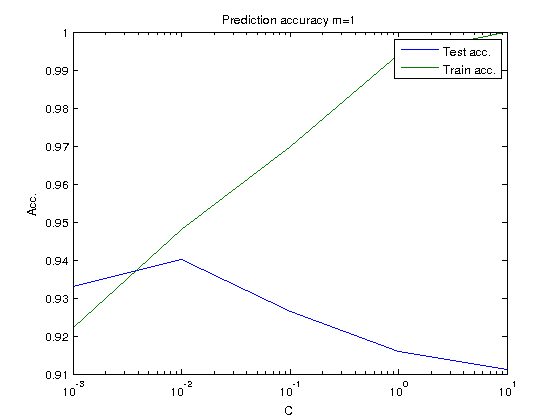
\includegraphics[width=9cm]{images/m1.png}}
	\subfloat[\label{fig:sub:2}]{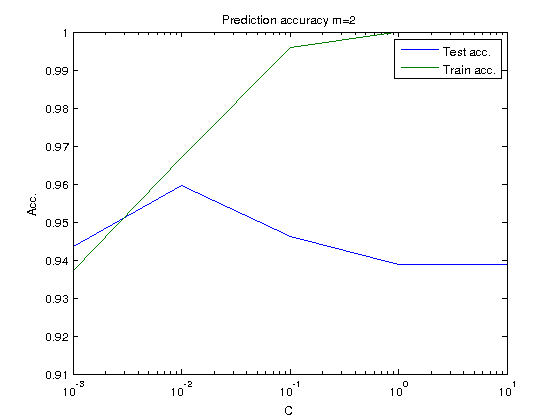
\includegraphics[width=9cm]{images/m2.png}}\\
	\subfloat[\label{fig:sub:3}]{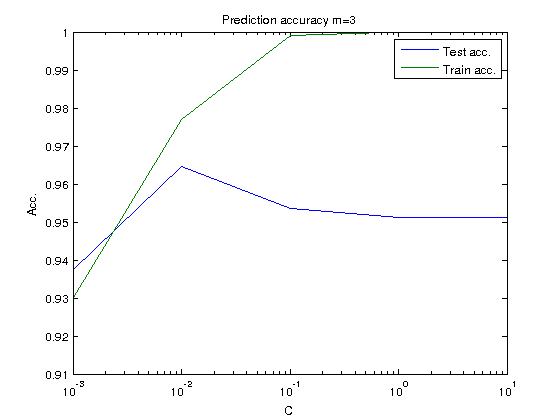
\includegraphics[width=9cm]{images/m3.png}}
	\caption{Prediction accuracy on testing and training data set depending on regularization constant $C$. Figure \protect\subref{fig:sub:1} $M=1$, figure \protect\subref{fig:sub:2} $M=2$ and figure \protect\subref{fig:sub:3} $M=3$.}
	\label{fig:ptacc}
\end{figure}

\begin{figure}
	\centering
	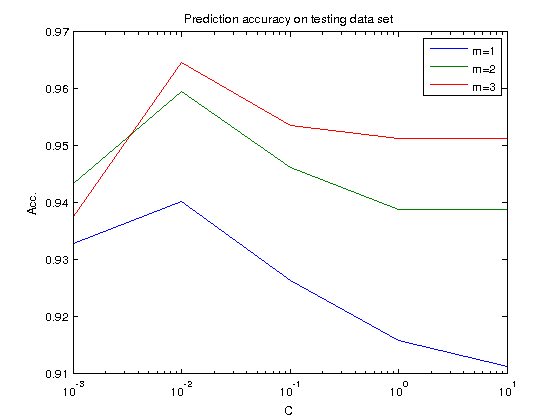
\includegraphics[width=12cm]{images/testing.png}
	\caption{Prediction accuracy on testing data set for all $m=1,2,3$ depending on the regularization constant $C$.}
	\label{fig:testing}
\end{figure}
\begin{table}
	\centering
	\subfloat[\label{tab:sub:1}]{
		\begin{tabular}{l|lll}
		\diaghead{We need}{$C$}{$M$}&$1$&$2$&$3$\\
		\hline
		$0.001$& $0.9329$ & $0.9434$ & $0.9375$ \\
		$0.01$ & $0.9402$ & $0.9595$ & $0.9646$ \\
		$0.1$ & $0.9264$ & $0.9462$ & $0.9536$ \\
		$1$ & $0.9159$ & $0.9389$ & $0.9513$ \\
		$10$ & $0.9113$ & $0.9389$ & $0.9513$
		\end{tabular}
	}
	\subfloat[\label{tab:sub:2}]{
		\begin{tabular}{l|lll}
		\diaghead{We need}{$C$}{$M$}&$1$&$2$&$3$\\
		\hline
		$0.001$& $0.922$ & $0.937$ & $0.93$ \\
		$0.01$ & $0.948$ & $0.967$ & $0.977$ \\
		$0.1$ & $0.97$ & $0.996$ & $0.999$ \\
		$1$ & $0.994$ & $1$ & $1$ \\
		$10$ & $1$ & $1$ & $1$
		\end{tabular}
	}
	\caption{Prediction accuracy \protect\subref{tab:sub:1} on testing data set and \protect\subref{tab:sub:2} on training data set.}
	\label{tab:data}
\end{table}


\end{document}
